\documentclass[tikz, border=1mm]{standalone}

\usetikzlibrary{positioning}

\begin{document}
	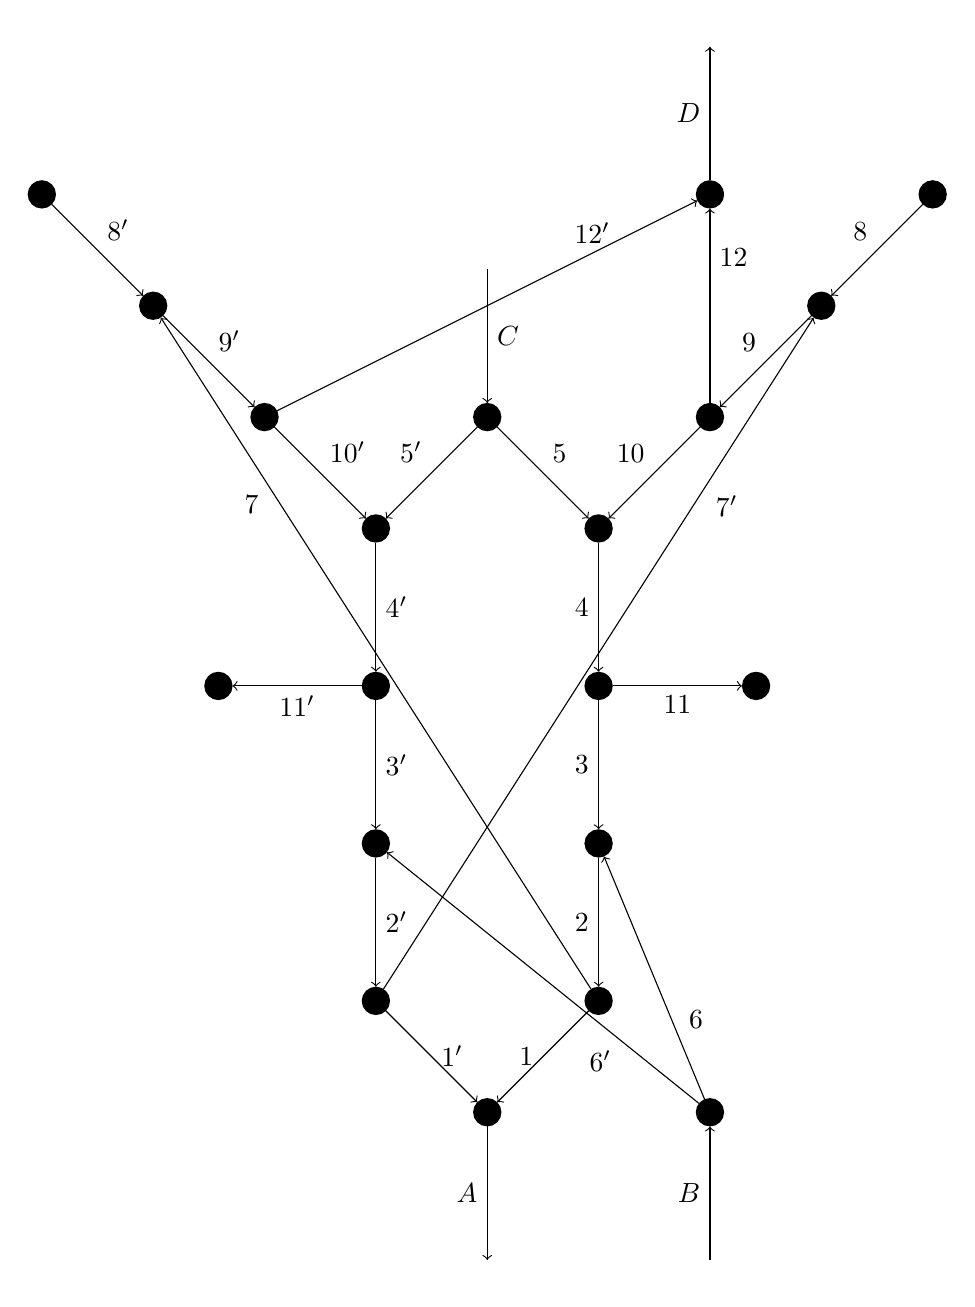
\begin{tikzpicture}[node distance={20mm}, main/.style = {draw, thick, circle, fill}]
		%% NODES
		% Start
		\node (1) {}; % Invisible start.
		\node[main, below of = 1] (2) {};
		% Left path
		\node[main, below left of = 2] (3) {};
		\node[main, below of = 3] (4) {};
		\node[main, below of = 4] (5) {};
		\node[main, below of = 5] (6) {};
		% Right path
		\node[main, below right of = 2] (3') {};
		\node[main, below of = 3'] (4') {};
		\node[main, below of = 4'] (5') {};
		\node[main, below of = 5'] (6') {};
		% End
		\node[main, below right of = 6] (7) {};
		\node[below of = 7] (8) {}; % Invisible end
		% Left wing		
		\node[main, above left of = 3] (9) {};
		\node[main, above left of = 9] (10) {};
		\node[main, above left of = 10] (11) {};
		% Right wing
		\node[main, above right of = 3'] (9') {};
		\node[main, above right of = 9'] (10') {};
		\node[main, above right of = 10'] (11') {};
		% Left arm
		\node[main, left of = 4] (12) {};
		% Right arm
		\node[main, right of = 4'] (12') {};
		% Rest of the graph.
		\node[main, above left of = 10'] (upper) {};
		\node[above of = upper] (ph-upper) {}; % Invisible upper
		\node[main, below right of = 6'] (lower) {};
		\node[below of = lower] (ph-lower) {}; % Invisible lower
		%% --S
		% Main two paths.
		\draw[->] (1) -- (2) node[midway, right] {$C$};
		\draw[->] (7) -- (8) node[midway, left] {$A$};
		\draw[->] (2) -- (3) node[midway, above left] {$5'$};
		\draw[->] (3) -- (4) node[midway, right] {$4'$};
		\draw[->] (4) -- (5) node[midway, right] {$3'$};
		\draw[->] (5) -- (6) node[midway, right] {$2'$};
		\draw[->] (6) -- (7) node[midway, right] {$1'$};
		\draw[->] (2) -- (3') node[midway, above right] {$5$};
		\draw[->] (3') -- (4') node[midway, left] {$4$};
		\draw[->] (4') -- (5') node[midway, left] {$3$};
		\draw[->] (5') -- (6') node[midway, left] {$2$};
		\draw[->] (6') -- (7) node[midway, left] {$1$};
		% Wings.
		\draw[->] (11) -- (10) node[midway, above right] {$8'$};
		\draw[->] (10) -- (9) node[midway, above right] {$9'$};
		\draw[->] (9) -- (3) node[midway, above right] {$10'$};
		\draw[->] (11') -- (10') node[midway, above left] {$8$};
		\draw[->] (10') -- (9') node[midway, above left] {$9$};
		\draw[->] (9') -- (3') node[midway, above left] {$10$};
		% Arms
		\draw[->] (4) -- (12) node[midway, below] {$11'$};
		\draw[->] (4') -- (12') node[midway, below] {$11$};
		% Rest of the graph.
		\draw[->] (ph-lower) -- (lower) node[midway, left] {$B$};
		\draw[->] (lower) -- (5) node[near start, below left]{$6'$};
		\draw[->] (lower) -- (5') node[near start, above right] {$6$};
		\draw[->] (upper) -- (ph-upper) node[midway, left] {$D$};
		\draw[->] (9) -- (upper) node[near end, above] {$12'$};
		\draw[->] (9') -- (upper) node[near end, right] {$12$};
		% The remaining two --s.
		\draw[->] (6) -- (10') node[near end, below right] {$7'$};
		\draw[->] (6') -- (10) node[near end, below left] {$7$};
	\end{tikzpicture}
\end{document}